\documentclass[a4paper]{article}
\usepackage{graphicx}


\title{\textbf{Dual Linear Regression Classification for Face Cluster Recognition}}
\date{}
\author{MANISH SHARMA - 2014A3PS181P\\Birla Institute of Technology and Science - Pilani \\ \texttt{f2014181@pilani.bits-pilani.ac.in}}

\begin{document}
	\maketitle
	
			
	\section{Result}
	
		\subsection{Database}
		For  DLRC, the database used for performance tests was LFW face database.
		
		LFW face database were captured in unconstrained environments
		such that there will be large variations in face images
		including pose,age, race, facial expression, lighting,
		occlusions, and background, etc. We use the aligned version
		of the LFW database, LFW-a database, to study the
		performance of the proposed classifiers. 
		
		All the
		images in LFW-a database are a size of 250 ${\times}$ 250. And for concentrating just on the faces and not the background, the images were cropped into
		a size of 90 ${\times}$78. A subset of LFW contains 62 persons,
		each people has more than 20 face images, is used for
		evaluating the algorithms. And in that, 10 images of each subject
		are selected to form the training set, while the last 10 image
		are used as the probe images.
		
		\begin{figure}[h!]
			
			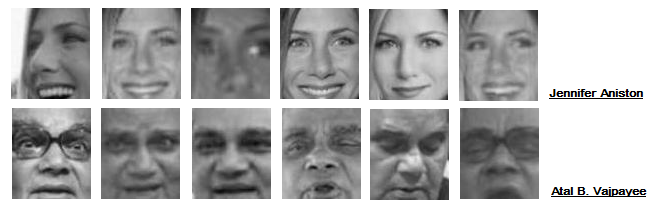
\includegraphics[scale=0.75]{sample_dataset.png}
			\caption{ Sample images of the processed lfw-a database }
			
			
		\end{figure}
		
		\subsection{Evironment used for Implementation}
		
		The operating system used is Windows 8.1  and programming is done on the software - MATLAB R2014a. 
		
				
		
			
			
			\subsection{Evaluation Criteria}
			The testing is done by passing the 62 face clusters (each having 10 images of the same person) from the test/probe set one by one to the DLRC classifier. And the predicted class is compared with the actual class of that cluster.
			
			\subsection{Observations}
			
			\begin{itemize}
				\item Correct predictions = 	58
				
				\item Total predictions		= 	62
				
				\item Accuracy of the DLRC classifier	=	93.55\%
			\end{itemize}
	
	\section{Conclusion}
						
			The Dual Linear Regression based Classifier (DLRC) for Facecluster Recognition MATLAB program was able to achieve an accuracy of 93.55\% for the image dimesnsions of $79\times91$. The accuracies obtained in the paper was 91.94\% for image dimensions $10\times10$ and 95.16\% for $15\times10$. 
			
			So the accuracy of this program was less than that presented in paper. The reason of that may be because in this project instead of manually cropping the image sets to get the most facial features, we automated the process using a seperate program for cropping.
			\begin{table}[h!]
				\centering
				\caption{Accuracy obtained compared with accuracies obtained from different image sizes in paper}
				
				\begin{tabular}{|l|l|l|l|}
					\hline
					Classifier    & $10\times10$ & $15\times10$ & \textbf{$79\times91$} \\ \hline
					\textbf{DLRC} & 91.94 & 95.16 & \textbf{93.55} \\ \hline
				\end{tabular}
			\end{table}
			
				
	\section{References}
	\begin{itemize}
		\item Chen, L., 2014. Dual linear regression based classification for face cluster recognition. In Proceedings of the IEEE Conference on Computer Vision and Pattern Recognition (pp. 2673-2680).
		
		\item Feng, Q., Zhou, Y. and Lan, R., 2016. Pairwise Linear Regression Classification for Image Set Retrieval. In Proceedings of the IEEE Conference on Computer Vision and Pattern Recognition (pp. 4865-4872).
		

	\end{itemize}
	
	
\end{document}